\documentclass{beamer}
\author{Miklos Vajna}

\setbeamertemplate{background canvas}[vertical shading][bottom=white,top=structure.fg!25]

\usetheme{Warsaw}
\setbeamertemplate{headline}{}
\setbeamertemplate{footline}[page number]
\setbeamersize{text margin left=0.5cm}
  
\usepackage[magyar, english]{babel}
\usepackage{times}
\usepackage[latin2]{inputenc}
\usepackage[T1]{fontenc}

\begin{document}

\title{GSoC project: Improving RTF Import \\ Presentation of a LibreOffice student}
\date{13 October 2011}

\frame{\titlepage}

\begin{frame}
\frametitle{Introduction}
\begin{itemize}
\item Background
\item Activities in LibreOffice earlier
\item Project this summer: development of a new RTF import filter
\begin{itemize}
\item developer side
\item user side
\end{itemize}
\end{itemize}
\end{frame}


\begin{frame}
\frametitle{Background}
\begin{itemize}
\item I'm a student from Budapest University of Technology and Economics, Hungary
\item A few project I am interested in:
\begin{itemize}
\item LibreOffice -- packaging, RTF filters
\item swig -- a binding generator
\item git -- I developed the current \texttt{git merge}
\item BitlBee -- an IM $\leftrightarrow$ IRC gateway
\item Frugalware Linux -- a distribution
\end{itemize}
\end{itemize}
\end{frame}

\begin{frame}
\frametitle{Activities in LibreOffice earlier}
\begin{itemize}
\item RTF export filter in Writer
\item Git-related patches
\item Packager for Frugalware Linux
\end{itemize}
\end{frame}

\begin{frame}
\frametitle{RTF Import Development}
\framesubtitle{Summary}
\begin{itemize}
\item The idea: RTF export is already subclassed from a generic Word exporter, the same could be done for the import
\item The \texttt{writerfilter} module already provides \texttt{dmapper} for common Word vs. Writer problems (e.g. field parsing)
\item Goal: support everything which was provided by the old filter, smaller size, new features
\end{itemize}
\end{frame}

\begin{frame}
\frametitle{RTF Import Development}
\framesubtitle{The big picture}
\begin{figure}[H]
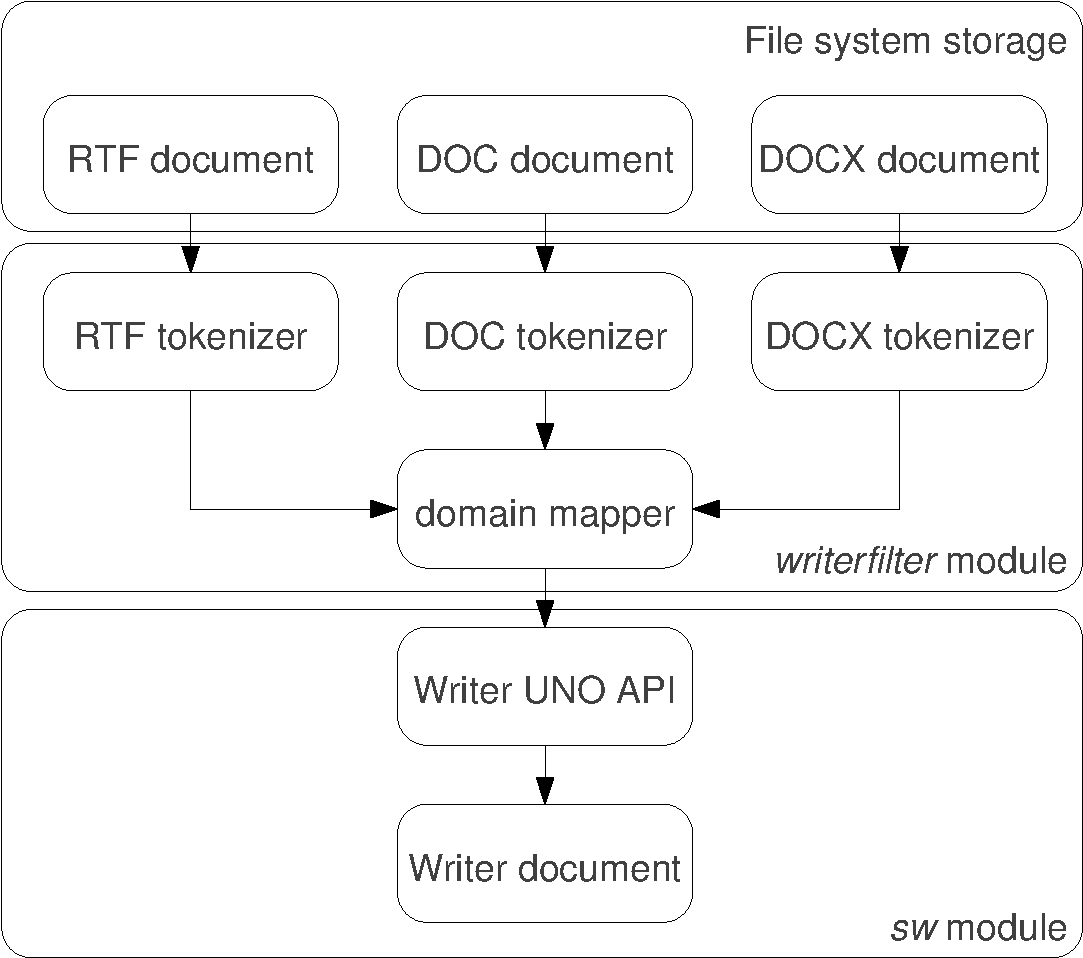
\includegraphics[width=225px,keepaspectratio]{pic/overview-architecture.pdf}
\end{figure}
\end{frame}

\begin{frame}
\frametitle{RTF Import Development}
\framesubtitle{Classes of the RTF import}
\begin{figure}[H]
\includegraphics[width=200px,keepaspectratio]{pic/rtf-classes.pdf}
\end{figure}
\end{frame}

\begin{frame}
\frametitle{RTF Import Development}
\framesubtitle{Testing}
\begin{itemize}
\item Created a unit test: it can quickly test if the tokenizer handles a document or not
\item Can be run without building the \texttt{sw} module, even
\item Does not replace manual testing (if the result visually matches the original)
\item Documents produced by OpenOffice.org 3.3, LibreOffice 3.4, Word 2007, Word 2010
\end{itemize}
\end{frame}

\begin{frame}
\frametitle{RTF Import New Features}
\framesubtitle{Nested tables}
Before:
\begin{figure}[H]
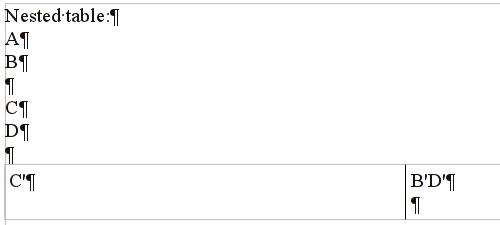
\includegraphics[width=200px,keepaspectratio]{pic/nested-old.png}
\end{figure}
After:
\begin{figure}[H]
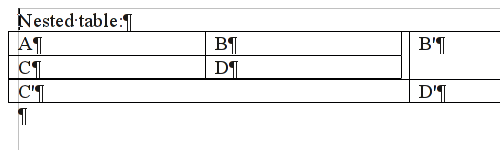
\includegraphics[width=200px,keepaspectratio]{pic/nested-new.png}
\end{figure}
\end{frame}

\begin{frame}
\frametitle{RTF Import New Features}
\framesubtitle{Footnotes}
\begin{itemize}
\item All characters of the foot/endnote mark are in the field
\item The field is properly superscripted
\item Before:
\begin{figure}[H]
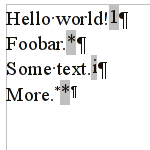
\includegraphics[width=75px,keepaspectratio]{pic/footnote-old.png}
\end{figure}
\item After:
\begin{figure}[H]
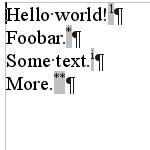
\includegraphics[width=75px,keepaspectratio]{pic/footnote-new.png}
\end{figure}
\end{itemize}
\end{frame}

\begin{frame}
\frametitle{RTF Import New Features}
\framesubtitle{Line numbering}
Before:
\begin{figure}[H]
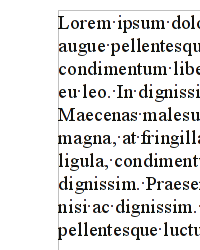
\includegraphics[width=50px,keepaspectratio]{pic/linenumbering-old.png}
\end{figure}
After:
\begin{figure}[H]
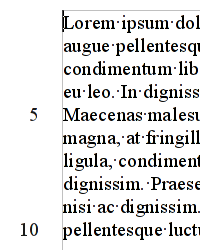
\includegraphics[width=50px,keepaspectratio]{pic/linenumbering-new.png}
\end{figure}
\end{frame}

\begin{frame}
\frametitle{RTF Import New Features}
\framesubtitle{Post-it fields}
Before:
\begin{figure}[H]

\includegraphics[width=250px,keepaspectratio]{pic/postit-old.png}
\end{figure}
After:
\begin{figure}[H]
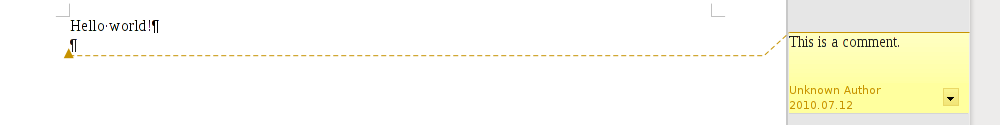
\includegraphics[width=250px,keepaspectratio]{pic/postit-new.png}
\end{figure}
\end{frame}

\begin{frame}
\frametitle{RTF Import New Features}
\framesubtitle{Form fields}
Before:
\begin{figure}[H]
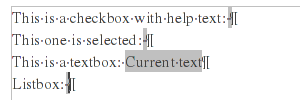
\includegraphics[width=100px,keepaspectratio]{pic/form-old.png}
\end{figure}
After:
\begin{figure}[H]
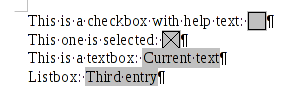
\includegraphics[width=100px,keepaspectratio]{pic/form-new.png}
\end{figure}
\end{frame}

\begin{frame}
\frametitle{RTF Import New Features}
\framesubtitle{Drawings}
Before:
\begin{figure}[H]
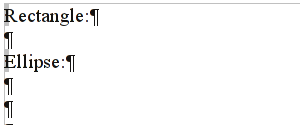
\includegraphics[width=100px,keepaspectratio]{pic/draw-old.png}
\end{figure}
\begin{figure}[H]

\includegraphics[width=100px,keepaspectratio]{pic/freeform-old.png}
\end{figure}
After:
\begin{figure}[H]
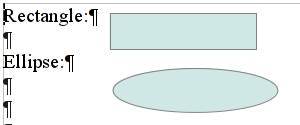
\includegraphics[width=100px,keepaspectratio]{pic/draw-new.png}
\end{figure}
\begin{figure}[H]

\includegraphics[width=100px,keepaspectratio]{pic/freeform-new.png}
\end{figure}
\end{frame}

\begin{frame}
\frametitle{RTF Import New Features}
\framesubtitle{Text frames}
Before:
\begin{figure}[H]
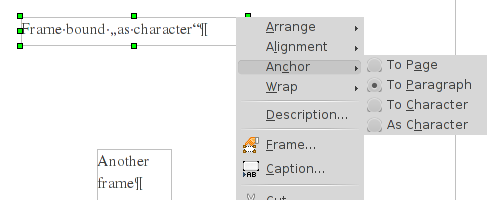
\includegraphics[width=150px,keepaspectratio]{pic/textframe-old.png}
\end{figure}
After:
\begin{figure}[H]
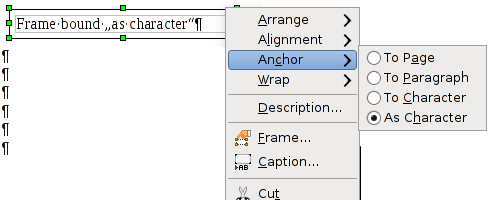
\includegraphics[width=150px,keepaspectratio]{pic/textframe-new.png}
\end{figure}
\end{frame}

\begin{frame}
\frametitle{DOCX Import Side-effects}
\framesubtitle{Footnote restart, extra paragraphs}
Before:
\begin{figure}[H]
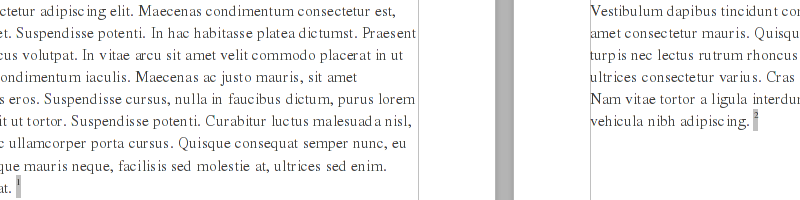
\includegraphics[width=200px,keepaspectratio]{pic/docx-footnote-restart-old.png}
\end{figure}
\begin{figure}[H]
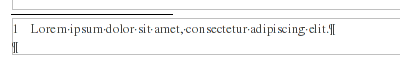
\includegraphics[width=100px,keepaspectratio]{pic/docx-footnote-par-old.png}
\end{figure}
After:
\begin{figure}[H]
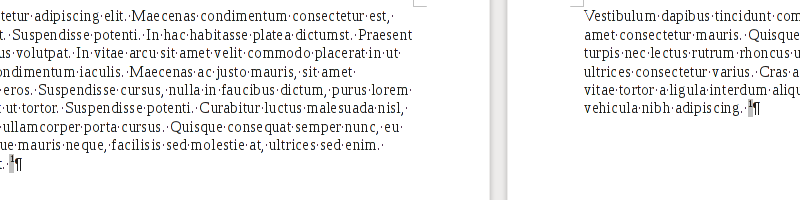
\includegraphics[width=200px,keepaspectratio]{pic/docx-footnote-restart-new.png}
\end{figure}
\begin{figure}[H]
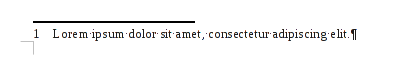
\includegraphics[width=100px,keepaspectratio]{pic/docx-footnote-par-new.png}
\end{figure}
\end{frame}

\begin{frame}
\frametitle{DOCX Import Side-effects}
\framesubtitle{Text-to-text alignment, double strikethrough}
Before:
\begin{figure}[H]
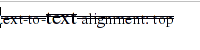
\includegraphics[width=50px,keepaspectratio]{pic/docx-text-to-text-old.png}
\end{figure}
\begin{figure}[H]
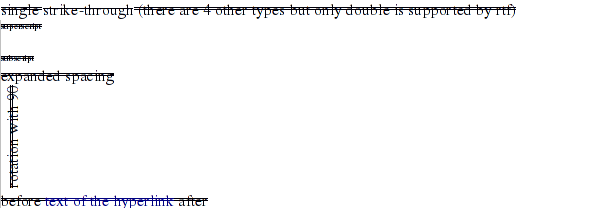
\includegraphics[width=175px,keepaspectratio]{pic/docx-strike-old.png}
\end{figure}
After:
\begin{figure}[H]
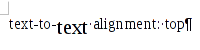
\includegraphics[width=50px,keepaspectratio]{pic/docx-text-to-text-new.png}
\end{figure}
\begin{figure}[H]
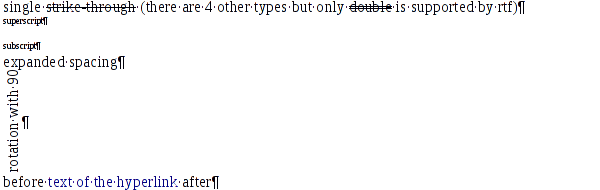
\includegraphics[width=175px,keepaspectratio]{pic/docx-strike-new.png}
\end{figure}
\end{frame}

\begin{frame}
\frametitle{Acknowledgements, References}
Thanks to -- in no particular order:
\begin{itemize}
\item C\'{e}dric Bosdonnat and Bj\"{o}rn Michaelsen: my mentors
\item Lubo\v{s} Lunak: writerfilter help
\item Michael Stahl: initial tokenizer help
\item Caol\'{a}n McNamara: unit test
\item Everyone else who helped on \texttt{\#libreoffice-dev}
\end{itemize}

References:
\begin{itemize}
\item LibreOffice: \url{http://www.libreoffice.org/}
\item SoC: \url{http://code.google.com/soc/}
\item New RTF import filter: \url{http://cgit.freedesktop.org/libreoffice/core/tree/writerfilter/source/rtftok}
\end{itemize}
\end{frame}

\end{document}
